\section{Experimental Setup}

The Long Beamline Neutrino Facility is the facility being internationally designed for the future Deep Underground Neutrino Experiment (DUNE) which has wide physics program for variety of precision measurements and searches beyond the Standard Model. The general scheme of the facility is shown on figure \ref{fig:LBNF_overallScheme}. This section gives more details on neutrino beam production and the detector descriptions. The information if taken mostly from the LBNF website[REFERENCE] and the Conceptual Design Report which is currenly under development but partially available [REFERENCE].

\begin{figure}
\caption{Long Baseline Neutrino Facility}
\label{fig:LBNF_overallScheme}
\centering
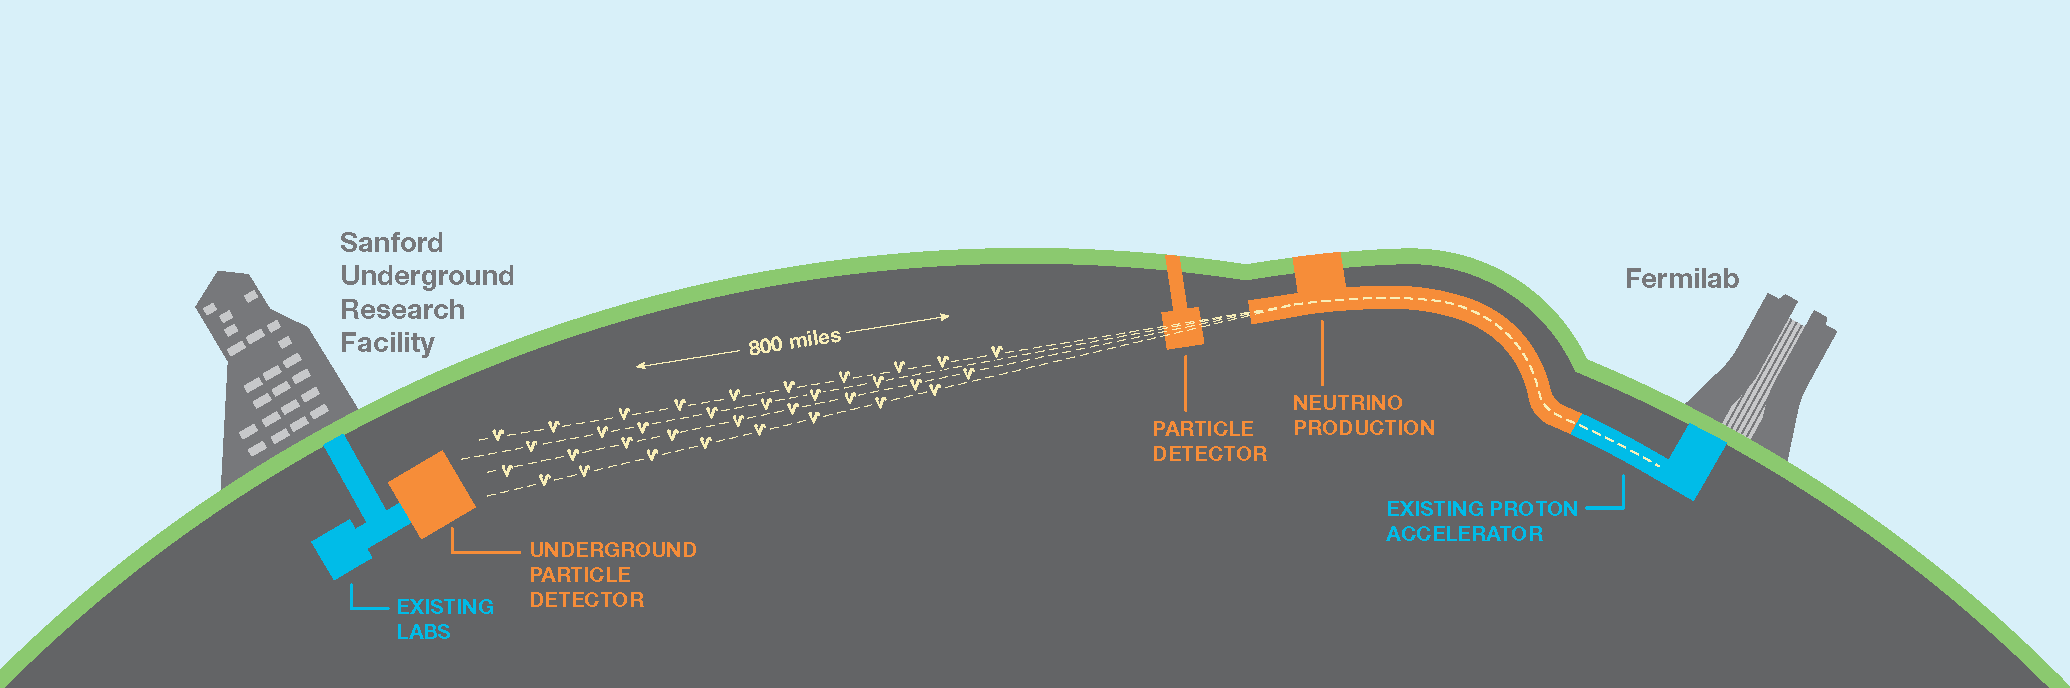
\includegraphics[width=0.95\textwidth, keepaspectratio=true]{figs/LBNF_overallScheme.png}
\\The neutrino flux will be produced using existing proton accelerator in Fermilab. Then neutrinos will be registered by close detector, travel 800 miles through the Earth mantle to the Sanford Underground Research Facility in South Dakota and be registed by far detector. \cite{ref_LBNFweb}   
\end{figure}

General requirements for the experiment are listed in [REFERENCE].
\begin{itemize}
  \item neutrino beam of high intensity which would be able to produce large amount of neutrinos to be registered at the far site
  \item the detector to register neutrinos and measure the beamline characteristics at the near site
  \item the liquid argon time-projection chamber for the far site detector (LArTPC)
\end{itemize}

\subsection{Neutrino Beam}

\begin{figure}
\caption{Neutrino beam of the LBNF}
\label{fig:LBNF_nuBeam}
\centering
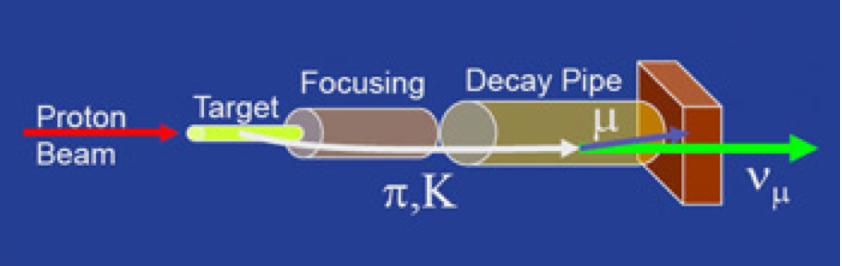
\includegraphics[width=0.45\textwidth, keepaspectratio=true]{figs/LBNF_nuBeam.png}
\\The neutrino beam production at Long Beamline Neutrino Facility. \cite{ref_LBNFweb}   
\end{figure}


\begin{figure}
\caption{Charged pion and kaon productions}
\label{fig:pionAndKaonProductions}
\centering
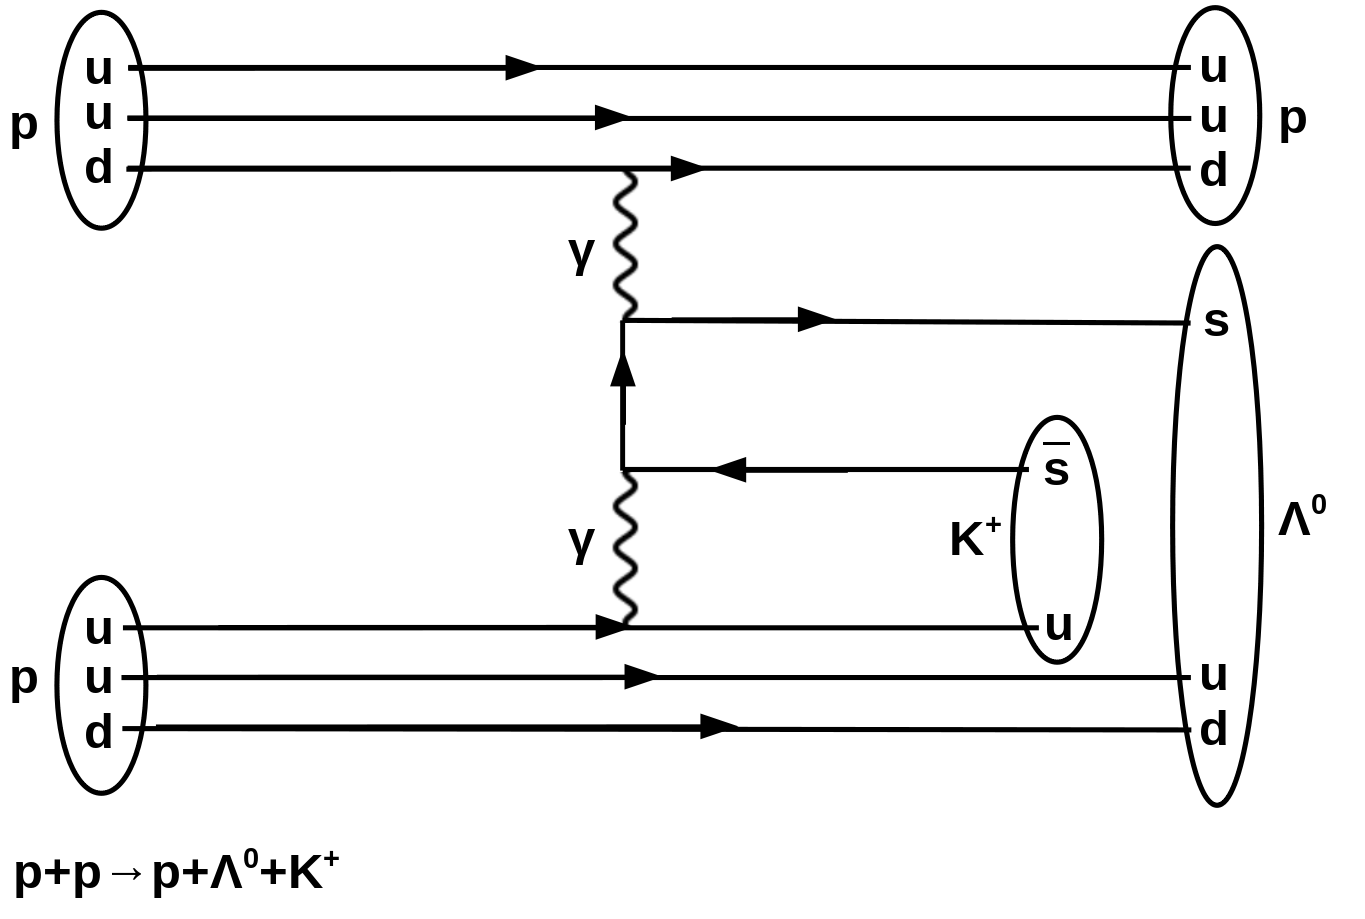
\includegraphics[width=0.48\textwidth, keepaspectratio=true]{figs/ppKaonProduction.png}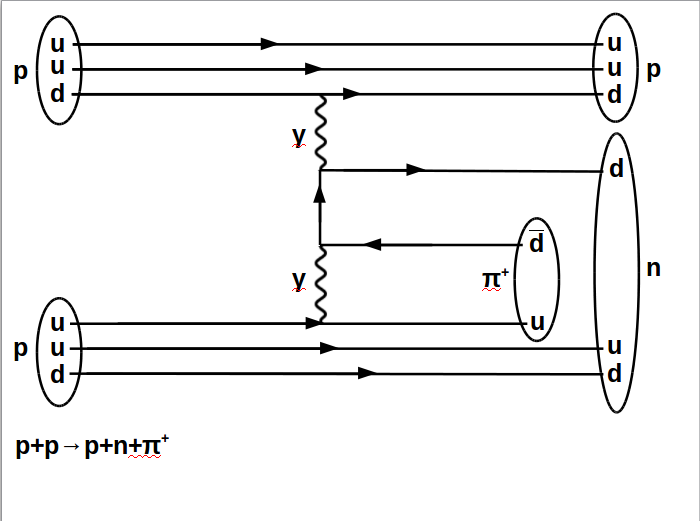
\includegraphics[width=0.48\textwidth, keepaspectratio=true]{figs/ppPionProduction.png}
\\Exmples of Feynmann diagrams of chagred kaons and pions production in proton-proton scattering.    
\end{figure}


It's going to use the highest intensity neutrino beam ever created. The proton accelerator in Fermilab which was already used in other experiments in Fermilab before will produce the beam of protons. Then protons will hit a target and create kaons and pions through the same reactions as take place in atmosphere when the cosmic protons hit molecules of air.  Pions can be created in the reactions $p+p \rightarrow p+n+\pi^+$, $p+p \rightarrow p+\Delta^{++}+\pi^-$, $p+n \rightarrow p+p+\pi^-$, $p+n \rightarrow n+n+\pi^+$, $p+n \rightarrow p+\Delta^{-}+\pi^+$ etc which go electromagnetically though photon. In more general words, one quark from the accelerator beam proton scatters on the other quark from the proton or neutron of the target substance. They exchange photon which produces quark-antiquark pair. At this moment, the system has seven quarks and one antiquark. The antiquark pairs up with one of the quarks participating in the reaction and the remaining six quarks make two baryons.  The charged pions have formulas $\pi^+ = u\bar{d}$ and $\pi^- = \bar{u}d$ and can be produced with the reactions which only include first generation quarks. The formulas of charged kaons are $K^+ = u\bar{s}$, $K^- = \bar{u}s$. Thus, to produce kaons, the photon has to produce $s\bar{s}$ pair. 

\begin{figure}
\caption{Charged pion and kaon decays}
\label{fig:pionAndKaonDecays}
\centering
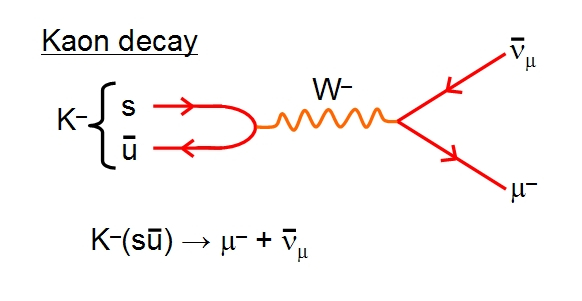
\includegraphics[width=0.45\textwidth, keepaspectratio=true]{figs/kaonDecay.jpg}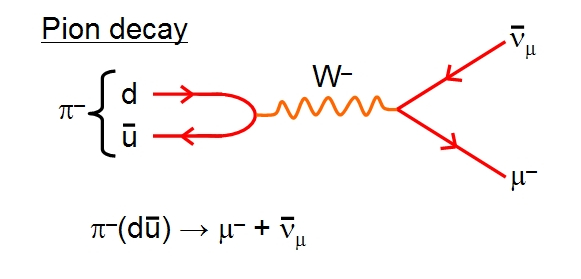
\includegraphics[width=0.45\textwidth, keepaspectratio=true]{figs/pionDecay.jpg}
\\Feynmann diagrams of charged pion and kaon decays to muon and muon antineutrino weakly through W-boson. Picture taken from \cite{ref_fig_pionandKaonDecays}.   
\end{figure}

After the mesons are created, they go through the focusing camera and decay into the decay pipe (the length of the decay pipe is about 200 meters) as $\pi^+ \rightarrow \mu^+\nu_\mu$, $\pi^- \rightarrow \mu^-\bar{\nu_\mu}$, $K^+ \rightarrow \mu^+\nu_\mu$, $K^- \rightarrow \mu^-\bar{\nu_\mu}$. The branching ratios of charged pions and kaons to decay into $\mu^+\nu_\mu$($\mu^-\bar{\nu_\mu}$) are $(>99.9)\%$ and $(63.55\pm0.011)\%$ respectively therefore most neutrinos produced into the decay pipe will be muon neutrinos. (While the neutral kaons can also be produced in the target and later decay in pions which could further decay and produce muon neutrinos, but the focusing is being done with the certain configuration of the magnetic field and thus only charged particles can be focused. Neutral pions, $\pi^0$s, are very likely to be produced as well but they decay as $\pi^0 \rightarrow \gamma\gamma$ and thus can't contribute to the neutrino production.)

After being produced in the rections described above, the neutrinos will be detected in the close detector in the Fermilab. Then the neutrinos will travel 800 miles underground and will be detected by Sanford Underground Research Facility in South Dakota.  

\subsection{Near Site Detector}

\subsection{Far Site Detector}
The Far Detector consists of 
\begin{itemize}
  \item Liquid Argon Time Projection Chamber (LArTPC)
  \item Data Aquisitin System (DAQ)
  \item Cold Electronics
  \item Photon Detector (PD)
\end{itemize}

\begin{figure}
\caption{LArTPC for the Far Detector of DUNE}
\label{fig:LBNF_TPC}
\centering
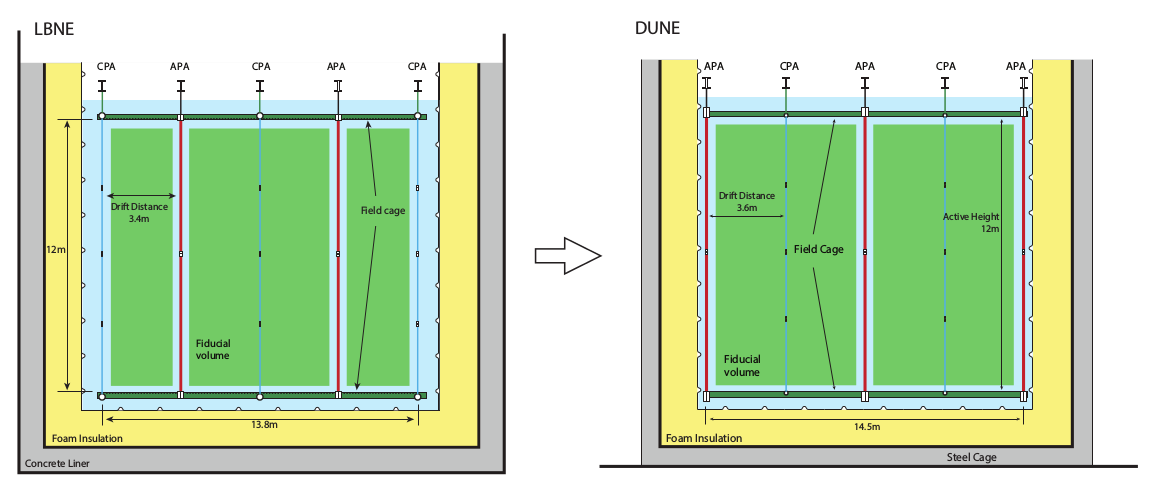
\includegraphics[width=0.85\textwidth, keepaspectratio=true]{figs/LBNF_TPC.png}
\\The scheme of the cross section of the LArTPC for far detector of the DUNE compared to LBNE (old experiment).   
\end{figure}

The TPC is particle identification system of the detector. The chamber is merged into the liquid argon at tempetature of 89 K. On the figure \ref{fig:LBNF_TPC} the cathod plane assemblies (CPAs) and the anode plane assemblies (APAs) are shown. The voltages on the APAs and the CPAs are applied in such a way to create unifoem electric field between anode and cathod planes. Chargedparticle traveling though the electron field ionizes argon atoms. Electrons induced in the ionization process drift to the APAs and produce signal on the readout electronic elements.
The important requirements to the TPC include:

\begin{itemize}
  \item be able to perform electron/photon discrimination
  \item wire sag shouldn't affect the position and energy resolutions
  \item discriminate electrons coming from photon conversion from primary electrons
  \item has good performance in measurements of high-energy and low-energy tracks
  \item make sure that materials used wouldn't contaminate high purity argon
\end{itemize}

The scheme of the data aquisition system is showm on figure \ref{fig:LBNF_DAQ}. The data aquisition is performed in two steps. First, data are triggered by software trigger farm. Then the data which passed trigger requirement are collected.

\begin{figure}
\caption{Block Diagram of the Data Aquisition System for the Far Detector of DUNE}
\label{fig:LBNF_DAQ}
\centering
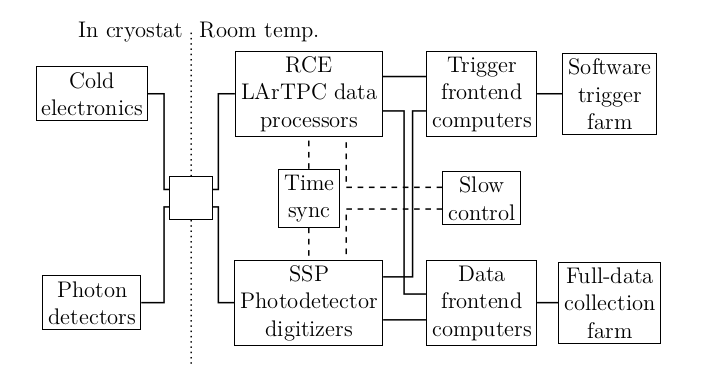
\includegraphics[width=0.70\textwidth, keepaspectratio=true]{figs/LBNF_DAQ.png}
%\\The scheme of the cross section of the LArTPC for far detector of the DUNE compared to LBNE (old experiment).   
\end{figure}
